%%%%%%%%%%%%%%
% The knitr process
% Christopher Gandrud
% Updated 3 January 2015
%%%%%%%%%%%%%%

% Define colors for figure
%% Color palette (GnBU) chosen using ColorBrewer 2.0
%% See: http://colorbrewer2.org/
%% Not used in the print version
\definecolor{Blue}{HTML}{7BCCC4}
\definecolor{LiteBlue}{HTML}{A8DDB5}
\definecolor{DarkBlue}{HTML}{08589E}

\definecolor{GrayLine}{HTML}{BDBDBD}

% Set node styles
%% Workflow stage nodes
\tikzstyle{Docs} = [draw=Blue,
                     rectangle,
                     inner sep=0.3cm,
                     font=\small]

% Begin tikz picture
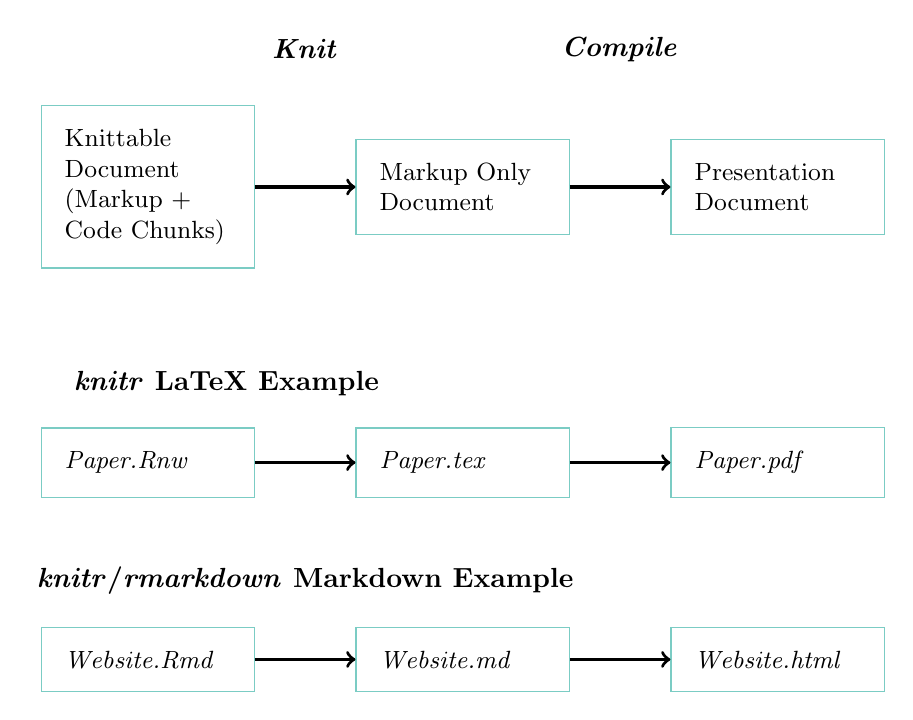
\begin{tikzpicture}

    \node(knit) at (2, 1.75) {{\emph{\textbf{Knit}}}};
    \node(compile) at (6, 1.75) {{\emph{\textbf{Compile}}}};

    % Document nodes
    \node (knittable) at (0, 0) [Docs, text width= 6em]{Knittable Document \\ (Markup + Code Chunks)};
    \node (Markup) at (4, 0) [Docs, text width= 6em]{Markup Only Document};
    \node (Presentation) at (8, 0) [Docs, text width = 6em]{Presentation Document};

    % LaTeX Example
    \node(LaTeX) at (1, -2.5) {\textbf{\emph{knitr} LaTeX Example}};
    \node (Rnw) at (0, -3.5) [Docs, text width= 6em]{\emph{Paper.Rnw}};
    \node (tex) at (4, -3.5) [Docs, text width= 6em]{\emph{Paper.tex}};
    \node (pdf) at (8, -3.5) [Docs, text width = 6em]{\emph{Paper.pdf}};

    % Markdown Example
    \node(Markdown) at (2, -5) {\textbf{\emph{knitr}/\emph{rmarkdown} Markdown Example}};
    \node (Rmd) at (0, -6) [Docs, text width= 6em]{\emph{Website.Rmd}};
    \node (md) at (4, -6) [Docs, text width= 6em]{\emph{Website.md}};
    \node (html) at (8, -6) [Docs, text width = 6em]{\emph{Website.html}};

    % Lines
    \draw [->, very thick] (knittable) -- (Markup);
    \draw [->, very thick] (Markup) -- (Presentation);

    \draw [->, very thick] (Rnw) -- (tex);
    \draw [->, very thick] (tex) -- (pdf);

    \draw [->, very thick] (Rmd) -- (md);
    \draw [->, very thick] (md) -- (html);

\end{tikzpicture}
